%!TEX root = ../sample.tex

\section{Related Work}
\label{sec:related}
\begin{figure}[t!]
	\centering
	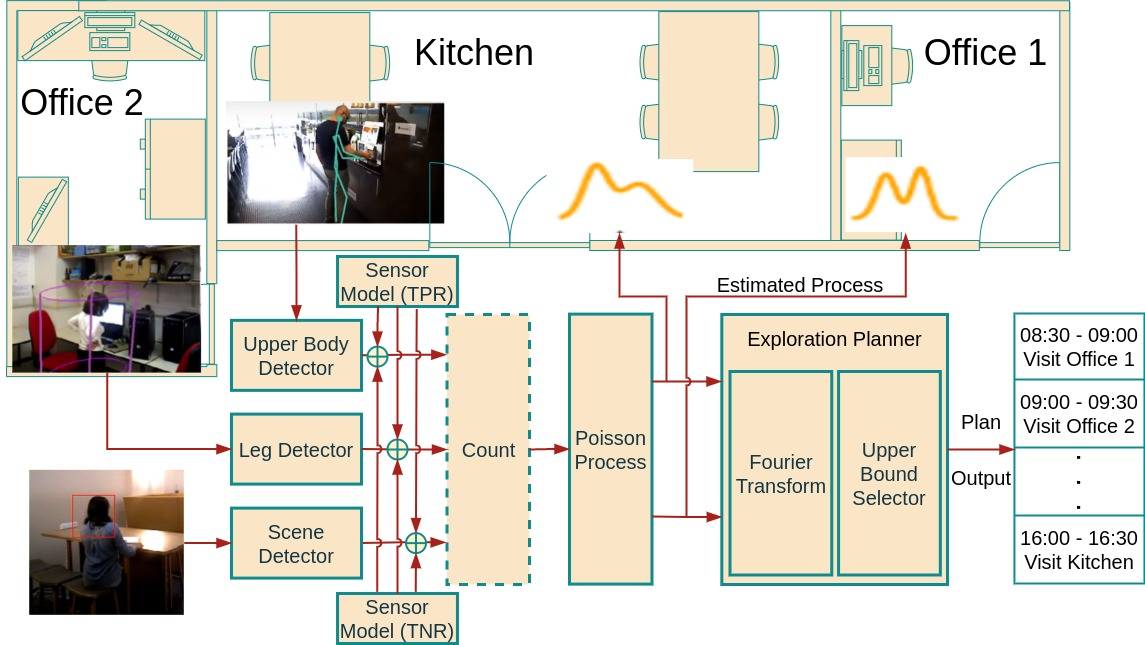
\includegraphics[width=0.8\textwidth]{./figures/popp_exploration_process.jpeg}
	\caption{A cycle process from count data collection, Poisson process estimation, through exploration plan generation for one day in an office-like environment. Count data are collected through perception algorithms or sensors while the robot patrols. The raw count data from multiple sensors are correctly filtered and merged via Bayesian inference taking into account the unreliability and correlation of each sensor to estimate the underlying Poisson process on each region of interest. Each estimate of the Poisson process is used by the exploration planner to find the maximum upper-bound of the Poisson process at each time interval and the corresponding region is chosen as a place to visit.} 
	\label{fig:popp_exploration_process_diagram}
	\vspace{-25pt}
\end{figure}
As requirements to employ the FOPP model are unlikely to be met, some existing works on statistical models propose a way to work with observation data that are not fully observable. In some literature, this is termed \emph{misclassified counts}. Misclassification happens when there are \emph{false positive counts} or \emph{false negative counts} (or both). False positive counts, also called the overcount, occur when the count includes events other than those of interest. False negative counts, also called the undercount, occur when some of the events of interest are missed. Work on the undercounting problem is common. Whittemore and Gong estimated cervical cancer rates by taking into account false negative data~\cite{whittemore1991}. Winkelmann and Zimmermann introduced a combination of a Poisson regression model with a logit model for under-counting, yielding the Poisson-Logistic (Pogit) model~\cite{winkelmann1993poisson}. They applied this to model the number of days employees were absent from a workplace. Dvorzak and Wagner adapted the Pogit model to use a small set of validation data, to provide information about the true counts~\cite{dvorzak2016}. They performed a Bayesian analysis of the Poisson-Logistic model and incorporate Bayesian variable selection to identify regressors with a non-zero effect and also to restrict parameters of the Poisson-Logistic model.

There is less prior work on the Poisson model for the case where the data may either be undercounted or overcounted~\cite{sposto1992,bratcher2002,bratcher2004,stamey2005}. Sposto et al. followed a frequentist approach to estimate both cancer and non-cancer death rates, assuming false negatives are possible on both sides of these counts~\cite{sposto1992}. In~\cite{bratcher2002}, Bratcher and Stamey used a Bayesian method to estimate Poisson rates in the presence of both undercounts and overcounts, borrowing the double sampling technique introduced in~\cite{Tenenbein1970}. They extended their work to a fully Bayesian method for interval prediction of the unobservable actual count in future samples, given a current double sample~\cite{bratcher2004}. Stamey and Young~\cite{stamey2005} present closed-form expressions for maximum likelihood estimators of the false negative rate, the false positive rate, and the Poisson rate for the model proposed in~\cite{bratcher2002}. The estimators are straightforward to calculate and to interpret in terms of evaluating the effectiveness of using unreliable counts.

Probabilistic approaches which do reason about sensing reliability have been applied to search and planning for robotics in a variety of settings. Many of them focus on optimization and maximization utilising the sensor model learned from observations in a continuous space. Velez et al. \cite{velez2012modelling} planned trajectories in a continuous space to maximize the reliability of object detection using a learned observation model. The key contribution is the use of a model of the correlations in sensor behaviour at nearby locations, thus driving the robot to gather more informative views. Martinez-Cantin et al. \cite{martinez2009bayesian} give a POMDP formulation of active visual mapping, use direct policy search to find a solution, and use Monte Carlo simulation to generate imaginary observations and action outcomes during optimization. The main challenge of decision-theoretic planning in partially observable environments is intractability. Kaplow et al. \cite{kaplow2010variable} employed a variable resolution map to achieve scaling with a robotic wheelchair. Task-level robot control with a decision-theoretic framework was first tackled by Pineau et al. \cite{pineau2003towards} using a POMDP planner to derive a high-level controller for a mobile robot with a dialogue system by exploiting hierarchy to reduce the state space.

What we propose is similar to that of Bratcher and Stamey~\cite{bratcher2002}. Both aim to accurately estimate the arrival rate parameter of a single Poisson process. Bratcher and Stamey utilise double sampling to obtain the true count together with false positive and false negative counts. They estimate the rate via MCMC since no closed form is found for $\lambda$, and the calculation of the full posterior is expensive. Double sampling assumes access to two counters with one always being a perfect counter. Our work goes beyond this since we consider multiple, potentially correlated, but always unreliable counters. We extend the work of Jovan et al in \cite{jovan18a} by presenting three extensions of our original model. We apply these extensions to the problem of robot exploration to optimize human robot-interactions. Similar to the work of Velez et al \cite{velez2012modelling} in utilizing sensor behaviours in driving the robot to gather more information, our work goes further by utilizing an exploration-exploitation mechanism provided by Bayesian optimization to maximize human interactions in the areas of interest.

% involved binomial and multinomial models~\cite{Bross1954,Chen1979,Hochberg1977,Tenenbein1970,Viana1993}. The first technique which was recorded to handle misclassification was double sampling. It was first introduced by Tenenbein to correct for misclassification of binomial data and obtain a maximum likelihood estimate~\cite{Tenenbein1970}. The double sampling approach utilizes two search techniques to retrieve relevant information: an expensive classification technique to obtain the true count along with the false positive count and false negative count from typically a small sample set, and a less-expensive classification technique only for error-prone counts on a larger sample set. The results of both counts are then combined to obtain estimators for the Poisson rate $\lambda$, and also for the misclassification parameters. The work of Tenenbein was then extended by Chen~\cite{Chen1979} and Hochberg~\cite{Hochberg1977} to correct misclassified counts in categorical and multinomial models to obtain maximum likelihood estimates. The double sampling technique was also extended to incorporate prior distributions in the binomial model and the posterior was obtained via Bayesian estimation~\cite{Viana1993}. Bekele extended the work of~\cite{Viana1993} by introducing a weighted prior scheme and allowing for several sources of information, including expert opinions~\cite{bekele1998binomial}.

% Different than the case of binomial and multinomial models, only a few studies are found working on the effect of partial observability of the data on the Poisson distribution. Many deal 
